% DOC SETTINGS ===================================
\documentclass{article}
\usepackage[utf8]{inputenc}
\usepackage{steinmetz}
\usepackage{mathtools}  
\usepackage{multicol}
\usepackage{circuitikz}
\usepackage{listings}
\usepackage{geometry}
\usepackage{indentfirst}
\usepackage{fancyhdr}
\pagestyle{fancy}
\usetikzlibrary{positioning, fit, calc}
\lhead{ECE2564 Project 3 Report}
\rhead{Kavin Thirukonda 2021}
\fancyheadoffset{0mm}
\title{Project 3 Report}
\author{Kavin Thirukonda\\
  Virginia Tech:  ECE2564\\
  Github ID: kavnthir
}
\date{April 2021}
 \geometry{
 a4paper,
 total={170mm,257mm},
 left=20mm,
 top=25mm,
 }
\mathtoolsset{showonlyrefs} 
% DOC SETTINGS ===================================
\begin{document}
\maketitle
\newpage
\section{Report Summary}
\indent
This report is meant to introduce the project, introduce the micro-controller that the project is being implemented on, and in addition talk about how the code to achieve the goals of the project is structured and organized.
\section{Project Description}
\indent
In this project, we had to develop a reaction time testing game on the MSP432P401R Launchpad. This required knowledge of finite state machines, the UART terminal, C programming, Interrupt based code architecture, and the Display residing on the Booster pack board. There are 3 main stages, splash screen, config screen and testing screen. In addition to this there is a high score screen. On the title screen the player is introduced to the title of the game the author, and shown a little picture to introduce the game. On the config screen the user picks the amount of trials they wish to happen and once every trial occurs an average of the trials are made. after this they are returned to the menu and prompted to redo if they wish. 
\begin{center}
    \boxed{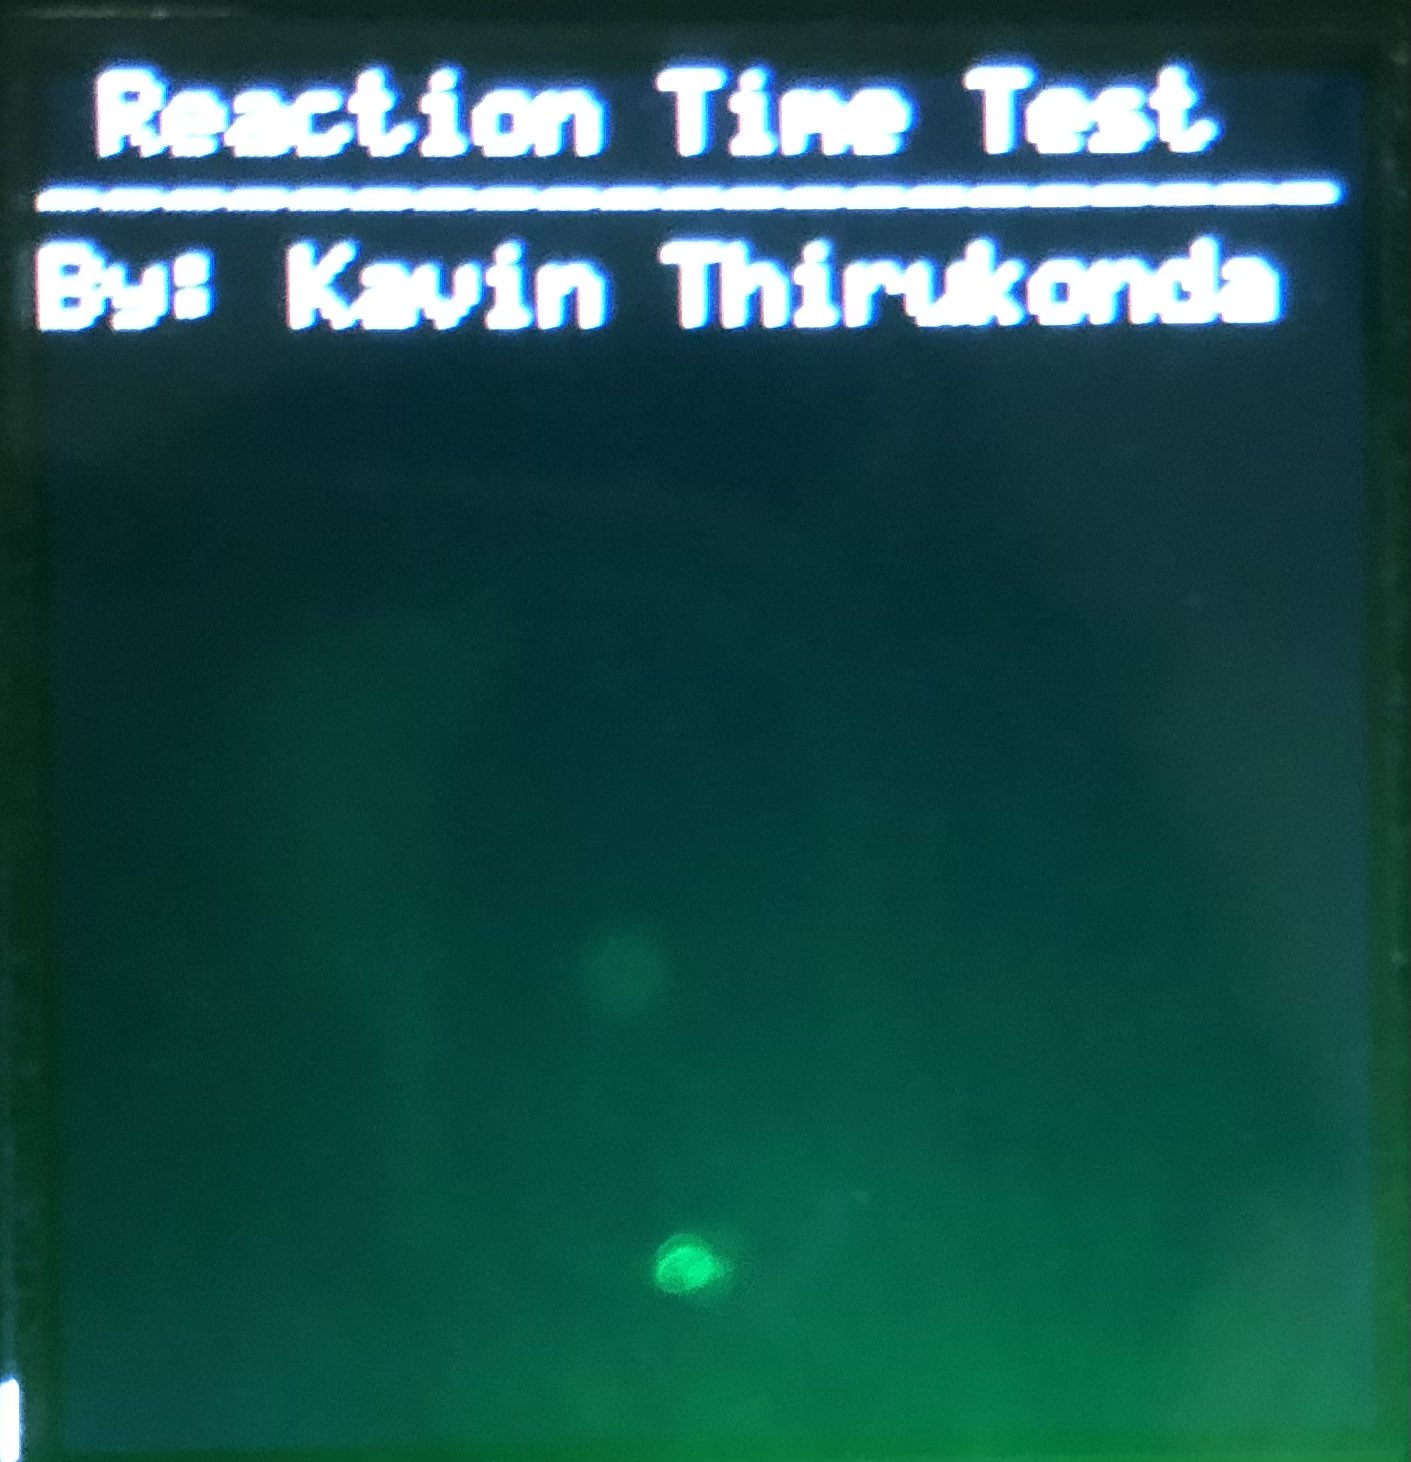
\includegraphics[width=.2\textwidth]{splash.jpg}}
    \boxed{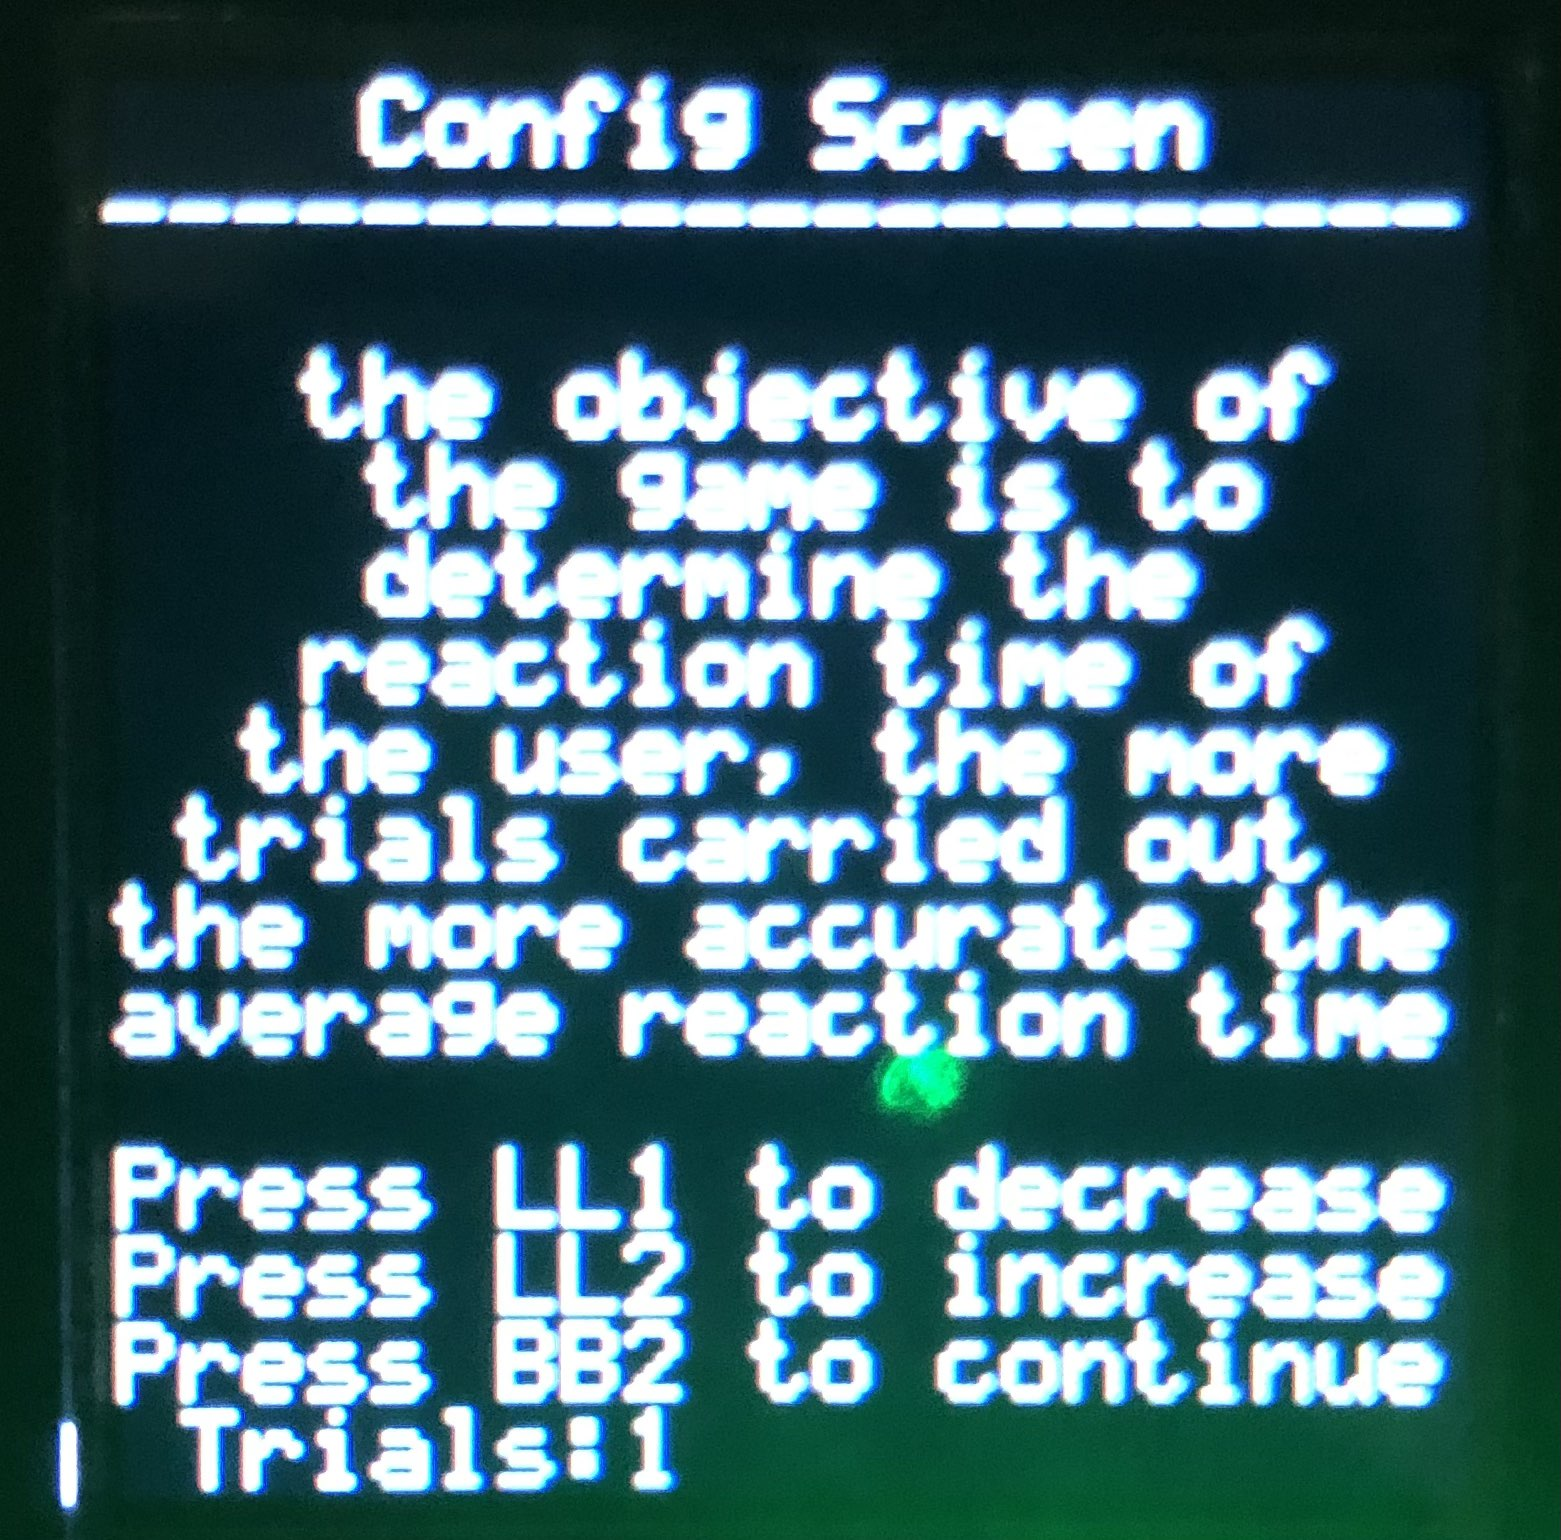
\includegraphics[width=.215\textwidth]{config.jpg}}
    \boxed{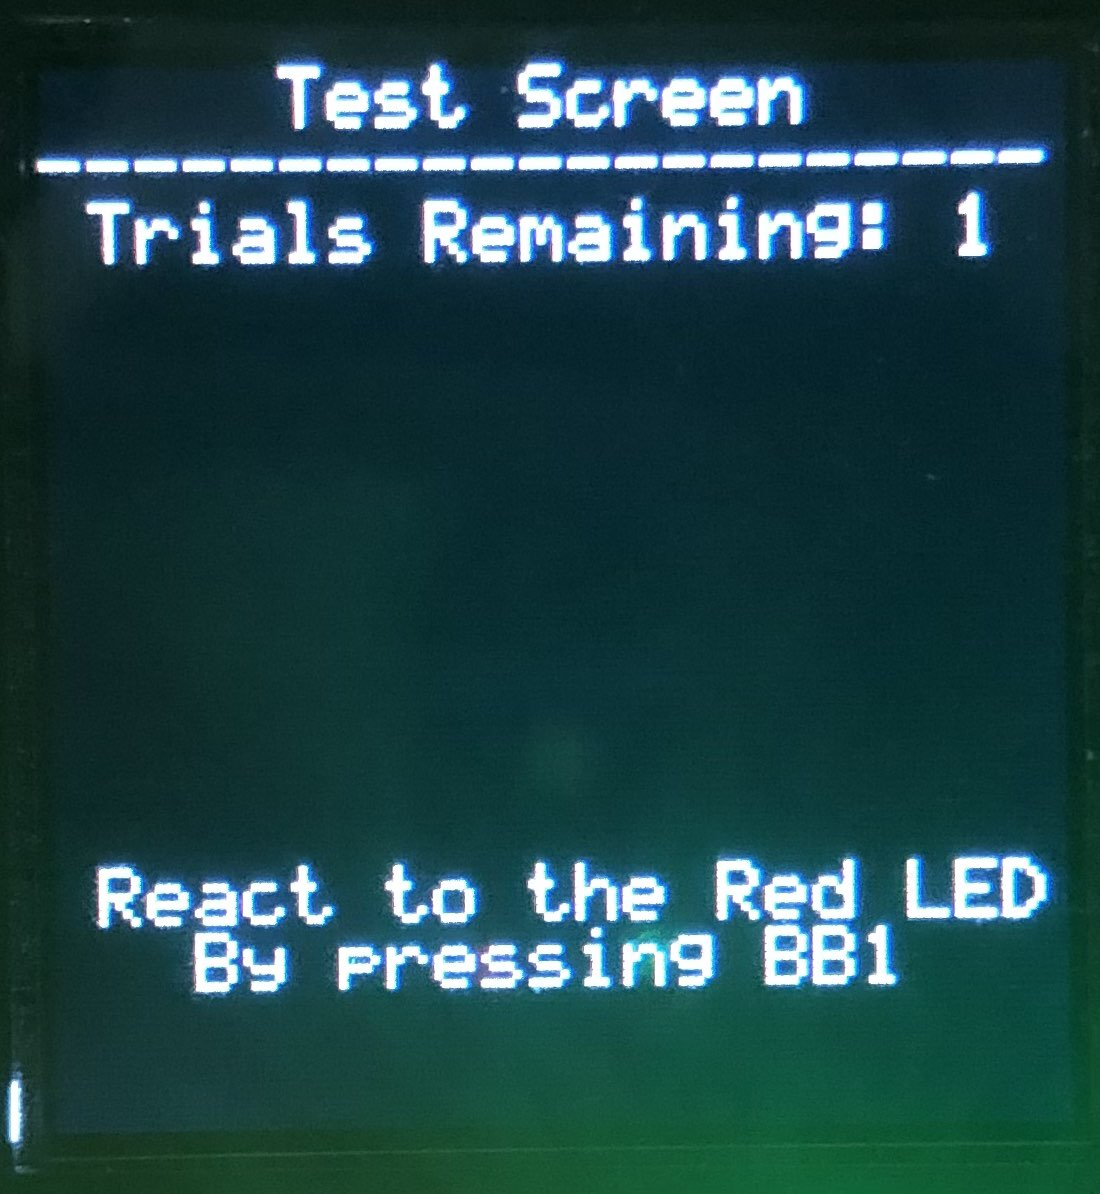
\includegraphics[width=.2\textwidth]{test.jpg}}
    \boxed{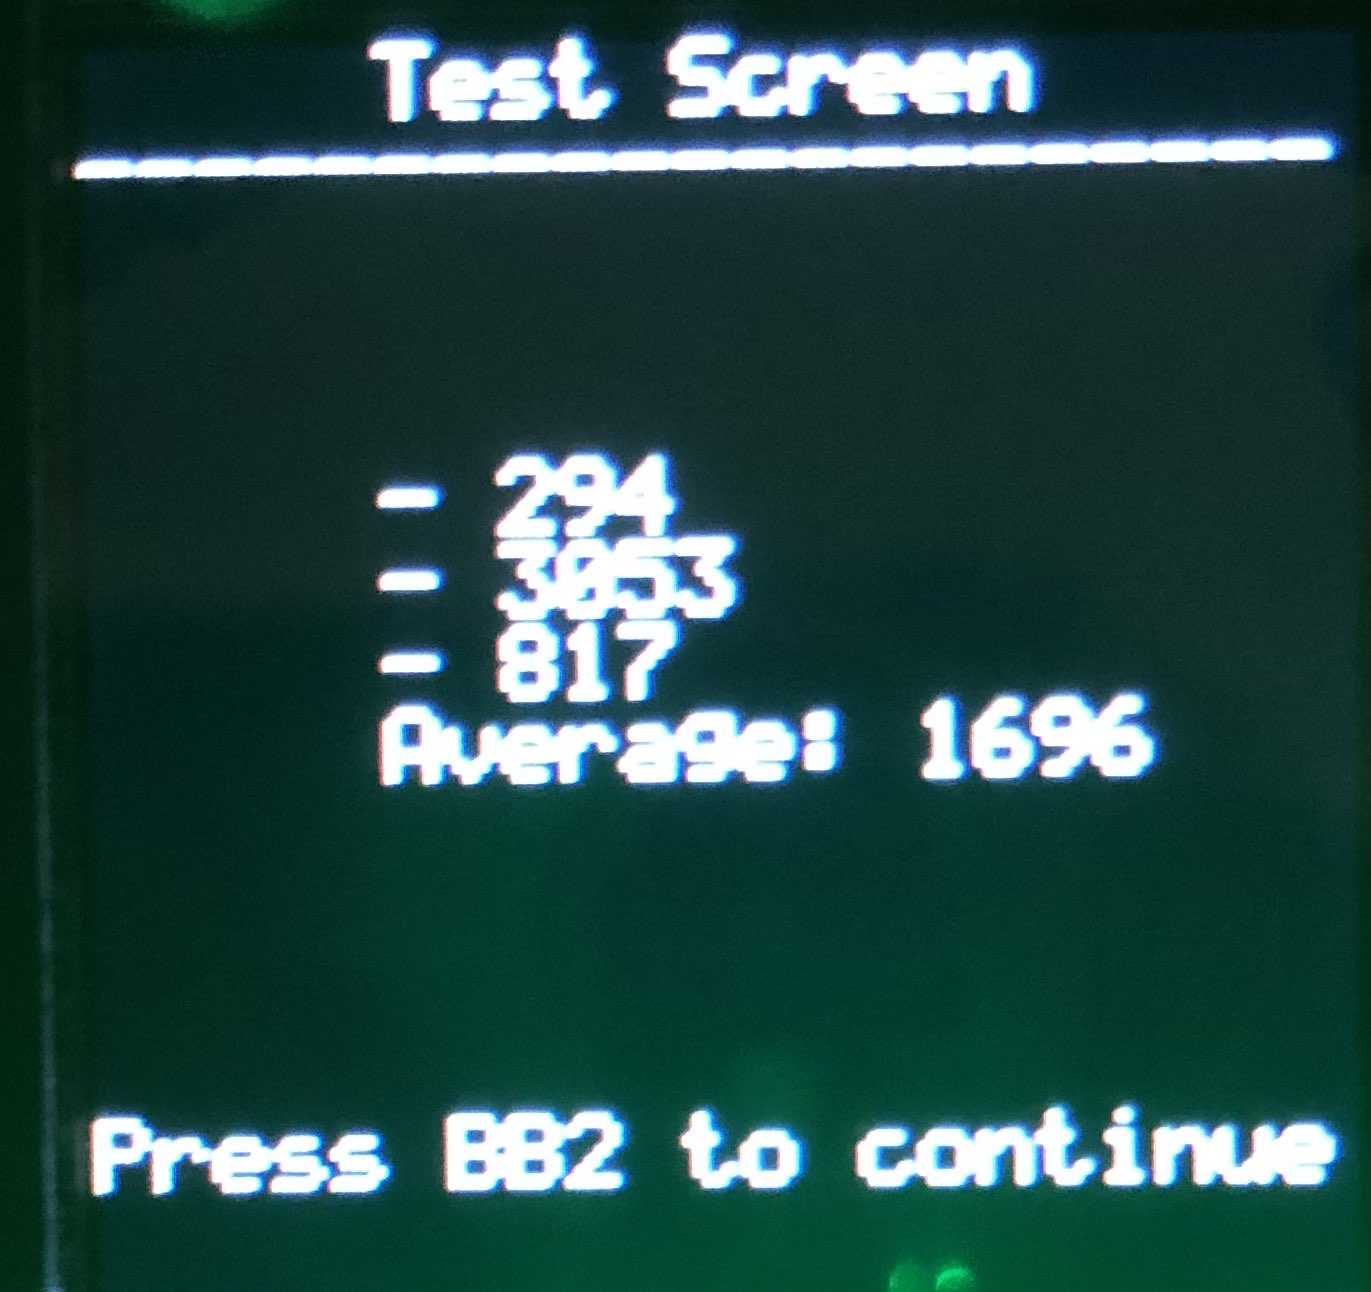
\includegraphics[width=.225\textwidth]{results.jpg}}
\end{center}

\section{Microcontroller-based embedded system architecture}
\begin{center}
    \begin{circuitikz}
    \draw (-2,0) node[draw,fill=pink,minimum width=40pt,minimum height=40pt](cpu){CPU}
    (-6,0) node[draw,fill=pink,minimum width=40pt,minimum height=40pt](msp){MSP}
    node[fit={(-3,-3)(3,3)},label={chip-level architecture},draw,inner sep=15pt]{}
    (-2,-2.5) node[draw,fill=pink,minimum size= 22.5pt](io1){I/O}
    (-1,-2.5) node[draw,fill=pink,minimum size= 22.5pt](io2){I/O}
    (0,-2.5) node[draw,fill=pink,minimum size= 22.5pt](io3){I/O}
    (1,-2.5) node[draw,fill=pink,minimum size= 22.5pt](io4){I/O}
    (2,-2.5) node[draw,fill=pink,minimum size= 22.5pt](io5){I/O}
    (0,2.5) node[draw,fill=pink,minimum size= 22.5pt](io6){I/O}
    (2,2.5) node[draw,fill=pink,minimum size= 22.5pt](io7){I/O}
    (0,1) node[draw,fill=pink,minimum width=30pt,minimum height=30pt](rx){$\begin{array}{c}euSCI\\RX\end{array}$}
    (2,1) node[draw,fill=pink,minimum width=30pt,minimum height=30pt](tx){$\begin{array}{c}euSCI\\TX\end{array}$}
    (cpu) to [short](io1)
    ($(cpu)+(.1,-.7)$) to [short]($(cpu)+(.1,-2)$)[short] to [short]($(cpu)+(1,-2)$)to[short]($(io2)+(0,.4)$)
    ($(cpu)+(.2,-.7)$) to [short]($(cpu)+(.2,-1.9)$)[short] to [short]($(cpu)+(2,-1.9)$)to[short]($(io3)+(0,.4)$)
    ($(cpu)+(.3,-.7)$) to [short]($(cpu)+(.3,-1.8)$)[short] to [short]($(cpu)+(3,-1.8)$)to[short]($(io4)+(0,.4)$)
    ($(cpu)+(.4,-.7)$) to [short]($(cpu)+(.4,-1.7)$)[short] to [short]($(cpu)+(4,-1.7)$)to[short]($(io5)+(0,.4)$)
    (io1) to [short,-*] ($(io1)+(0,-1.03)$) node[anchor=north]{P1.0}
    (io2) to [short,-*] ($(io2)+(0,-1.03)$) node[anchor=north]{P1.1}
    (io3) to [short,-*] ($(io3)+(0,-1.03)$) node[anchor=north]{P1.2}
    (io4) to [short,-*] ($(io4)+(0,-1.03)$) node[anchor=north]{P3.5}
    (io5) to [short,-*] ($(io5)+(0,-1.03)$) node[anchor=north]{P2.0}
    ($(rx)+(0,-.55)$) to [short]($(cpu)+(2,0)$) to [short](cpu)
    ($(tx)+(0,-.55)$) to [short]($(cpu)+(4,-.1)$) to [short]($(cpu)+(.71,-.1)$)
    (io6) to[short](rx)
    (io7) to[short](tx)
    ($(io6)+(0,.4)$) to [short]($(io6)+(0,.8)$) to [short,-*]($(io6)+(3.53,.8)$)node[anchor=west]{P1.3}
    ($(io7)+(0,.4)$) to [short]($(io7)+(0,.5)$) to [short,-*]($(io7)+(1.53,.5)$)node[anchor=west]{P1.2}
    node[fit={(-11,-3)(-5,3)},label={board-level architecture},draw,inner sep=15pt]{}
    (-6,2)node[draw,circle,fill=pink](ll1){LB1}
    (-7.25,2)node[draw,circle,fill=pink](ll2){LB1}
    (-8.5,2)node[draw,circle,fill=pink](jsb){BB2}
    (-9.75,2)node[draw,circle,fill=pink](bb1){BB1}
    (-6,-3.5)node[draw,fill=pink,minimum width=20pt,minimum height=20pt](usb){USB} to [short]
    (-6,-2.5)node[draw,fill=pink,minimum width=20pt,minimum height=20pt](xds){XDS} to [short]
    (-6,-1.5)node[draw,fill=pink,minimum width=20pt,minimum height=20pt](iso){Isolation}
    (msp) to [short] (ll1);
    \draw ($(iso)+(.2,.34)$) to [short]($(iso)+(.2,.78)$);
    \draw ($(iso)+(-.2,.34)$) to [short]($(iso)+(-.2,.78)$);
    \draw ($(msp)+(-.1,.7)$) to [short]($(msp)+(-.1,1.4)$) to [short]($(msp)+(-1.25,1.4)$) to [short]($(msp)+(-1.25,1.5)$);
    \draw ($(msp)+(-.2,.7)$) to [short]($(msp)+(-.2,1.3)$) to [short]($(msp)+(-2.5,1.3)$) to [short]($(msp)+(-2.5,1.5)$);
    \draw ($(msp)+(-.3,.7)$) to [short]($(msp)+(-.3,1.2)$) to [short]($(msp)+(-3.75,1.2)$) to [short]($(msp)+(-3.75,1.5)$);
    \draw (-10,0) node[draw,fill=pink,minimum width=35pt,minimum height=35pt](lcd){LCD} to[short](msp);
    \draw (-1.8,-1.225) node[draw,fill=pink,minimum width=20pt,minimum height=10pt]{IRQ};
    \end{circuitikz}
\end{center}
\begin{center}
    Assuming the two boards we have are one, the architecture of this system is quite simple, since a very low amount of inputs from the actual boards are used, most inputs come from the joystick, there is also UART which gets used for a bonus point opportunity which is probably the most complicated part about the architecture.
\end{center}
\newpage
\section{Code Quality}
\subsection{Comments}
\begin{center}
    The comments in my code show what each function does, the input and output of each function, and whenever a chunk of code is called there is a brief explanation of when the code will be called and what happens when the code does get called. 
\end{center}
\subsection{No Global Variables}
\begin{center}
    The only global variables used are the ones used for images which according to specification are allowed
\end{center}
\subsection{No Numeric Values}
\begin{center}
    all values are defined using macros, which explain the meaning of the number
\end{center}
\subsection{No Long Functions}
\begin{center}
    All functions are below max length and line number commented at the top of relevant functions.
\end{center}
\subsection{Using HAL} 
\begin{center}
    The HAL were used properly when needed.
\end{center}
\subsection{Non-Blocking Code}
\begin{center}
    In all places of the code the blocking test did in fact turn on the LED and therefore the code is nonblocking.
\end{center}
\begin{center}
    \begin{tabular}{c|c}
         Code Quality Aspect &  Expected Points\\
         \hline
         Comments & 10\\
         No Global Variables & 20\\
         No Numeric Values & 20\\
         No Long Functions & 30\\
         Non-Blocking Code & 20\\
    \end{tabular}
\end{center}
\end{document}
